\subsection{Esquema de dependências}

\begin{figure}[H]
	\centering
	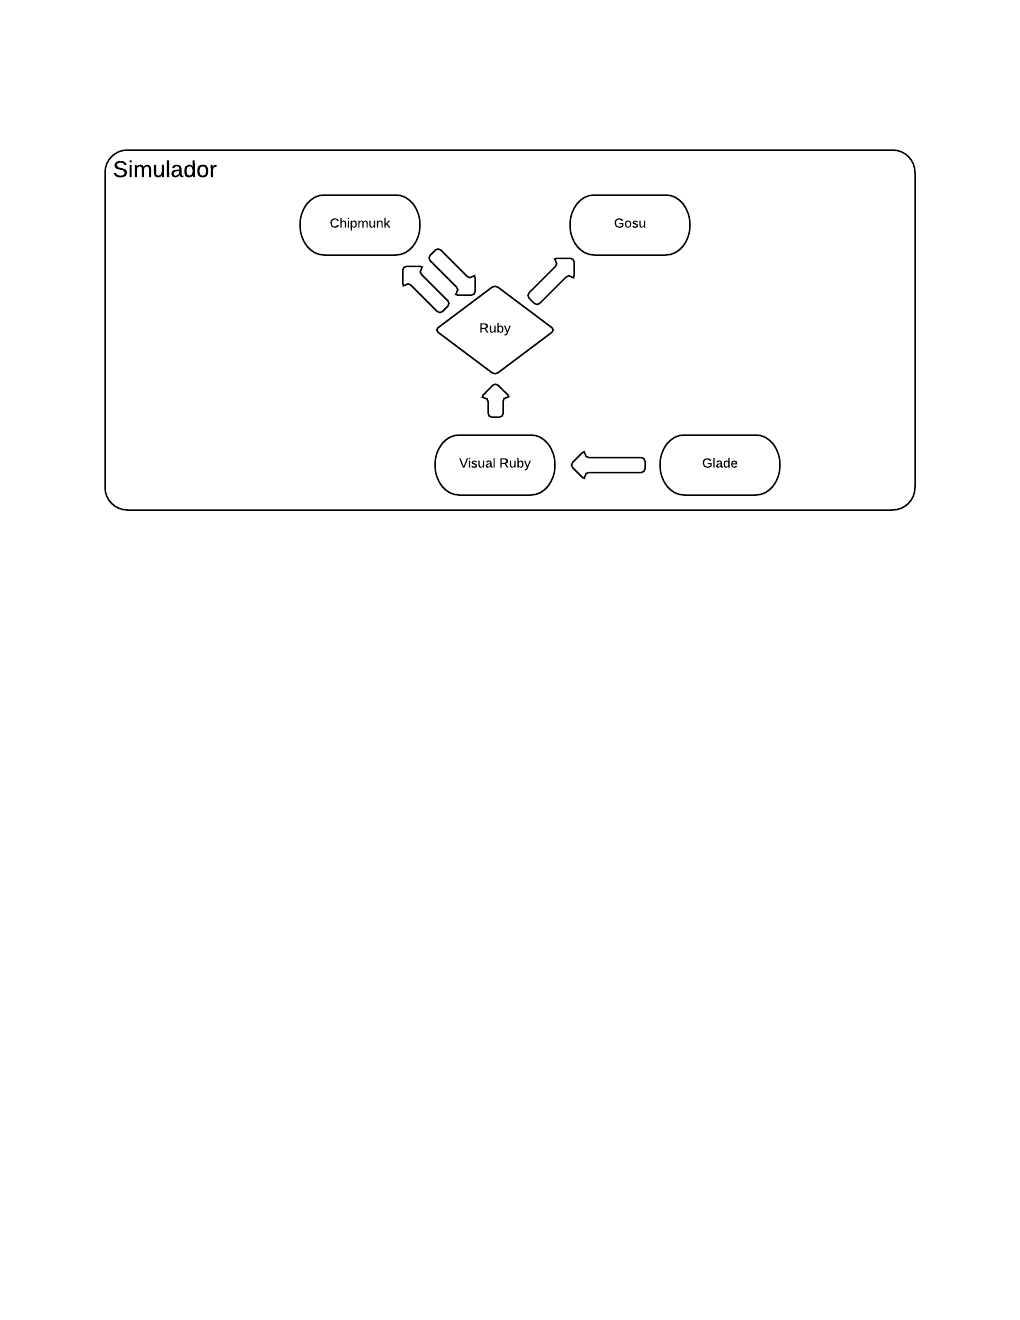
\includegraphics[scale=0.45]{images/esquema-dependencias.png}
	\caption{Dependências do Physimulation}
\end{figure}

\subsection{Ruby}
É a linguagem de programação utilizada no simulador. A sintaxe foi baseada no Pearl e Smalltalk e é uma linguagem interpretada com tipagem dinâmica e forte. \\ 

Algumas das características da linguagem são:
\begin{itemize}
  \item Mostrar códigos e alguns itens interessantes do ruby
\end{itemize}

Explicar sobre gem.

\subsection{Simulação com Chipmunk}
Chipmunk é uma biblioteca física 2D escrita em C. Esta biblioteca permite criar objetos convexos e segmentos que se interagem em um ambiente físico com algumas propriedades 
como por exemplo a gravidade. \\

Para utilizar esta biblioteca é preciso criar as formas dos objetos (Shapes), associá-los a um corpo (Body) e adicioná-los ao ambiente físico (Space).
TODO: Explicar melhor cada conceito com codigos. \\

Existe uma versão do Chipmunk portado para a linguagem Ruby.

\subsection{Animação com Gosu}
A animação é feita com o Gosu, uma biblioteca para desenvolvimento de jogos em 2D em Ruby e C++. Fornece somente as seguintes funcionalidades:

\begin{itemize}
  \item Criação de uma janela com um laço principal e callbacks
  \item Criação de textos e imagens 2D
  \item Som e música em vários formatos
  \item Tratamento de eventos de entrada de teclado e mouse
\end{itemize}

TODO: Mostrar exemplos com codigos

\subsection{Cenários com Glade}
Glade é uma ferramenta que facilita o desenvolvimento de interfaces de usuário em formato de XML. A interface inicial do usuário foi criado com Glade.\\

TODO: Falar melhor do Glade, visualruby e mostrar exemplos de código
\subsection{Exemplo}

Mostrar codigos da simulação.
